%%%%%%%%%%%%%%%%%%%%%%%%%%%%%%%%%%%%%%%%%
% University/School Laboratory Report
% LaTeX Template
% Version 3.0 (4/2/13)
%
% This template has been downloaded from:
% http://www.LaTeXTemplates.com
%
% Original author:
% Linux and Unix Users Group at Virginia Tech Wiki 
% (https://vtluug.org/wiki/Example_LaTeX_chem_lab_report)
%
% License:
% CC BY-NC-SA 3.0 (http://creativecommons.org/licenses/by-nc-sa/3.0/)
%
%%%%%%%%%%%%%%%%%%%%%%%%%%%%%%%%%%%%%%%%%

%----------------------------------------------------------------------------------------
%	PACKAGES AND DOCUMENT CONFIGURATIONS
%----------------------------------------------------------------------------------------

\documentclass{article}

\usepackage[version=3]{mhchem} % Package for chemical equation typesetting
\usepackage{siunitx} % Provides the \SI{}{} command for typesetting SI units

\usepackage[top=1in, bottom=1in, right=1in, left=1in]{geometry}

%Add code formating
\usepackage{listings}
\lstset{tabsize=2}

\usepackage{hyperref}

\usepackage{amssymb}

\usepackage{enumerate}

%Add extra support for image placement
\usepackage{float}

%\usepackage{mcode}

\usepackage{graphicx} % Required for the inclusion of images

\setlength\parindent{0pt} % Removes all indentation from paragraphs

\renewcommand{\labelenumi}{\alph{enumi}.} % Make numbering in the enumerate environment by letter rather than number (e.g. section 6)

% Setup how hyperlinks look
\usepackage{xcolor}
\hypersetup{
    colorlinks,
	linkcolor={red!50!black},
	citecolor={blue!50!black},
	urlcolor={blue!80!black},
}


% Create a new command to format code
\def\code#1{\textbf{\texttt{#1}}}



%\usepackage{times} % Uncomment to use the Times New Roman font

%----------------------------------------------------------------------------------------
%	DOCUMENT INFORMATION
%----------------------------------------------------------------------------------------

\title{Keysight Hacking Platform Getting Started} % Title

\author{Blake \textsc{Vermeer}} % Author name

\date{\today} % Date for the report

\begin{document}

\maketitle % Insert the title, author and date

\begin{center}
\begin{tabular}{l r}
Date Performed: & September 18, 2017 \\ % Date the experiment was performed
Company: & Keysight Technologies % Company
\end{tabular}
\end{center}

% If you wish to include an abstract, uncomment the lines below
% \begin{abstract}
% Abstract text
% \end{abstract}

%----------------------------------------------------------------------------------------
%	OVERVIEW
%----------------------------------------------------------------------------------------
\section{Overview}

This document gives an brief overview of the hardware in the Keysight Hacking Platform (KHP), how to connect the the KHP over SSH, and where to find the example programs.   \\

The KHP consists of:

	\begin{itemize}
		
		\item Raspberry Pi 3 with 2.8" capacitive touch screen shield
		
		\item Raspbian Linux image with some example programs pre-loaded.
		
		\item Some additional hardware to hack with (ADC, resistors, LEDs, sensor modules)
		
	\end{itemize}

The general workflow for using the KHP consists of connecting to it over Secure Shell (SSH) and transferring files using Session Control Protocol (SCP).

	\begin{figure}[H]
		\centering
		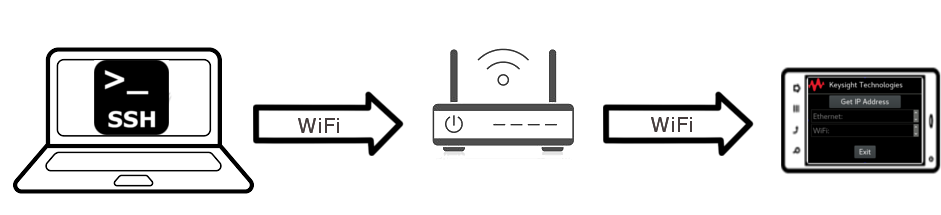
\includegraphics[scale=0.5]{pics/Deployment_Workflow.png}
		\caption{KHP Deployment Workflow}
		\label{KHP_App_Deployment}
	\end{figure}



%----------------------------------------------------------------------------------------
%	Connecting to the Raspberry Pi Over SSH
%----------------------------------------------------------------------------------------
\section{Connecting to the Raspberry Pi Over SSH}

The Raspberry Pi will take approximately a minute to boot up after plugging it in. After fulling booting up the Raspberry Pi will automatically start the Keysight IP Finder application. Click the \textbf{Get IP Address} button to show the configured IP addresses for the Ethernet and WiFi interfaces. Depending on how quickly the interface receives an IP address you may have to click the button a few times.

	\begin{figure}[H]
		\centering
		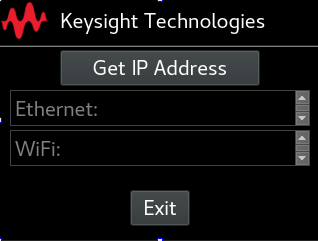
\includegraphics[scale=0.75]{pics/Show_IP_app.png}
		\caption{Keysight Show IP App}
		\label{Show_IP_app}
	\end{figure}

Write down the IP address of the interface you would like to use. We are now going to use this IP address to connect to the Raspberry Pi over SSH. Follow the instructions for the operating system running on your computer:

	\begin{center}
		\textbf{SSH Login Credentials}
	\end{center}
	\begin{center}
		\begin{tabular}{| c | c |}
			\hline
			Username: & \textbf{pi} \\
			\hline
			Password: & \textbf{keysight} \\
			\hline
		\end{tabular}
	\end{center}



	\subsection{Windows}
	
		\begin{enumerate}[1.)]
			\item Download and install the PuTTY program if you do not have it already. Link: \href{https://www.chiark.greenend.org.uk/~sgtatham/putty/latest.html}{PuTTY}
			
			\item Launch the PuTTY program.
				
				\begin{figure}[H]
					\centering
					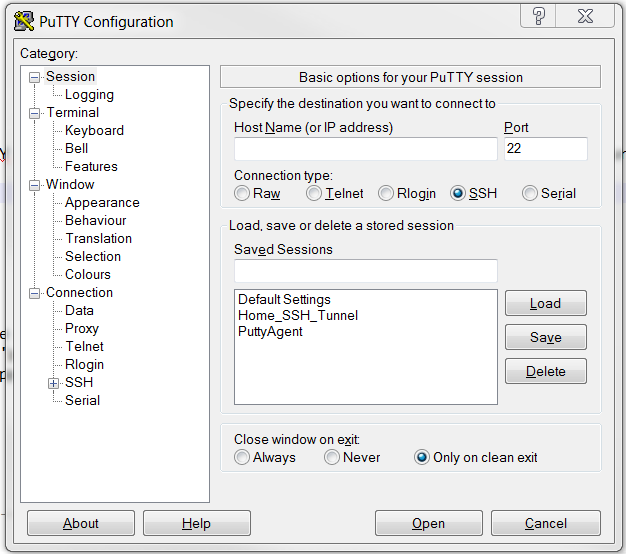
\includegraphics[width=\textwidth / 2]{pics/PuTTY.png}
					\caption{PuTTY Application}
					\label{Show_IP_app}
				\end{figure}
			
			\item Type in the IP address you wrote down in the previous section in the \textbf{Host Name} box and make sure the \textbf{SSH} option is selection under "Connection Type:" and then click the \textbf{Open} button.
			
			\item Type in \textbf{pi} as the user name and then press enter.
			
			\item Type in \textbf{keysight} as the password and then press enter.
			
			\item At this point you will be dropped into a Bash command prompt on the Raspberry Pi.
			
		\end{enumerate}
	
	\subsection{Mac OS X and Linux}
	
		\begin{enumerate}[1.)]
			\item Open up a terminal
			
			\item Using the IP address you wrote down in the previous step, type in: \code{ssh pi@\{IP Address\}}
			
			\item Type in the password for the 'pi' user and press enter: \textbf{keysight}
			
			\item At this point you will be dropped into a Bash command prompt on the Raspberry Pi.
			
		\end{enumerate}





%----------------------------------------------------------------------------------------
%	Finding and Running the Example Programs
%----------------------------------------------------------------------------------------
\section{Finding and Running the Example Programs}

All of the example programs are located in folders under this location:

	\begin{center}
		\begin{tabular}{| l | c |}
			\hline
			\textbf{Example Program Location:} & \code{/home/pi/Documents/Hackathon/} \\
			\hline
		\end{tabular}
	\end{center}

All of the example programs are Python programs. To run any of the example programs, change into the directory with the example program you wish to run (\code{cd}) and then run: \code{python \{Example Program Name\}}. To stop running the example program press \code{Ctrl+C} on your keyboard to end the program.




%----------------------------------------------------------------------------------------
%	Transferring files with SCP
%----------------------------------------------------------------------------------------
\section{Transferring files with SCP}

Files can be transferred to and from the Raspberry Pi using the SCP protocol. Follow the directions below for the operating system that you are using.


	\subsection{Windows}
	
	To be able to transfer files to and from the Raspberry Pi using Windows, we first need to download and install the WinSCP program.
	
	
		\begin{enumerate}[1.)]
			\item Download and install the \href{https://winscp.net/download/WinSCP-5.11.1-Setup.exe}{WinSCP} program.
			
			\item After installing the WinSCP program, launch the program. You will be presented with the login screen which will look similar to Figure \ref{WinSCP_Login}.
			
				\begin{figure}[H]
					\centering
					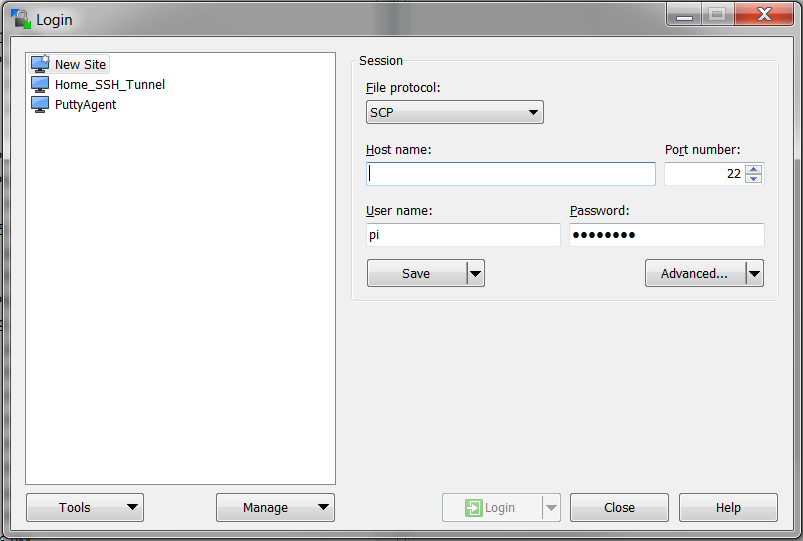
\includegraphics[width=\textwidth / 2]{pics/WinSCP_login.png}
					\caption{WinSCP Login Screen}
					\label{WinSCP_Login}
				\end{figure}
			
			\item In the File Protocol drop-down box, select \textbf{SCP}.
			
			\item In the "Host Name" box, enter the IP address of your Raspberry Pi.
			
			\item In the "User name" box, enter \textbf{pi}.
			
			\item In the "Password" box, enter \textbf{keysight}
			
			\item Click the \textbf{login} button. At this point you should be connected to the Raspberry Pi and be able to browse the Raspberry Pi's file system and transfer files.
			
		\end{enumerate}
	

	
	
	\subsection{Mac OS X}
	
	With Mac OS X there are a few different ways that you can go about using SCP with the Raspberry Pi. You can either use the SCP utility from the command line for transferring files or you can download and install MacFusion to allow you to browse the Raspberry Pi's file system through Finder.
	
	
	\subsection{Linux}



%----------------------------------------------------------------------------------------
%	APPENDIX
%----------------------------------------------------------------------------------------

%\newpage
%\section{Appendix}

%\begin{enumerate}

	
%	\item[1. a.)] \lstinputlisting{../MATLAB/problem_1a.m}
	

%\end{enumerate}






%----------------------------------------------------------------------------------------


\end{document}